\documentclass[12pt]{article}
\usepackage{graphicx}
\usepackage{amsmath}
\usepackage{hyperref}
\usepackage{geometry}
\geometry{margin=1in}
\usepackage{float}
\title{HW3 Report: KNN Regressor}
\author{Thomas Meltesen}
\date{\today}

\begin{document}

\maketitle


This report documents the results and conclusions for the application of a KNN Regressor on a dataset.


\section{Introduction}
Experiment with KNN regression using Python in combination with in lecture
discussed ML, data processing, and data visualization packages.

\section{Data Description}
The Homework 3 Data was loaded from a csv which contained 500 samples of 3 continuous features: X1, X2 and X3, which were predictors of the output Y. 


\subsection{Dataset Overview}
The 500 sample dataset from the Homework 3 csv was loaded using pandas then split:
% Table: Data Split Summary
\begin{table}[ht]
\centering
\begin{tabular}{|c|c|c|}
\hline
Set & X Shape & Y Shape \\
\hline
Training (50\%)   & (250, 3) & (250, 1) \\
Validation (20\%) & (100, 3) & (100, 1) \\
Test (30\%)       & (150, 3) & (150, 1) \\
\hline
\end{tabular}
\caption{Data Split: Training, Validation, and Test Sets}
\label{tab:data_split}
\end{table}

\subsection{Preprocessing}
Since KNN Regressor's work by calculating for instance a distance metric from it's respective neighborhood the data was fitted and transformed using sklearn's StandardScaler to reduce its $\mu=0$ and $\sigma^2 = 1$. To prevent the local neighborhood from being to 'far' from the values we want to predict.

\section{Results}
Results of considering different data splits with random state = 42 and 24. Tables in (3.1 parts A-F) and (3.3 part G) show the values for each instance state and the best K (highlighted). The visualizations in (3.2 parts A-F) and (3.4 part G) show the curves for $R^2$ score in train/val/test.
\subsection{$R^2$ vs K for Parts A-F}
% Table: R^2 Scores for K=1 to 15
\begin{table}[H]
\centering
\begin{tabular}{|c|c|c|c|}
\hline
K & R$^2$ Train & R$^2$ Validation & R$^2$ Test \\
\hline
1  & 1.000000 & 0.600257 & 0.644254 \\
2  & 0.896969 & 0.702868 & 0.720414 \\
3  & 0.866707 & 0.694269 & 0.734280 \\
4  & 0.840770 & 0.702921 & 0.739007 \\
\textbf{5}  & \textbf{0.840457} & \textbf{0.715831} & \textbf{0.717467} \\
6  & 0.811066 & 0.701440 & 0.702668 \\
7  & 0.793847 & 0.694601 & 0.691904 \\
8  & 0.787908 & 0.678408 & 0.656656 \\
9  & 0.769049 & 0.691797 & 0.649328 \\
10 & 0.752338 & 0.684485 & 0.643712 \\
11 & 0.733712 & 0.681662 & 0.634182 \\
12 & 0.723468 & 0.673014 & 0.622918 \\
13 & 0.707985 & 0.661187 & 0.598688 \\
14 & 0.693134 & 0.651491 & 0.583700 \\
15 & 0.681376 & 0.635325 & 0.568710 \\
\hline
\end{tabular}
\caption{R$^2$ Scores for KNN Regression (K=1 to 15) for random state = 42. The best validation score is at $\mathbf{K=5}$.}
\label{tab:r2_scores_42}
\end{table}


\subsection{Visualizations Parts A-F}
\begin{figure}[H]
    \centering
    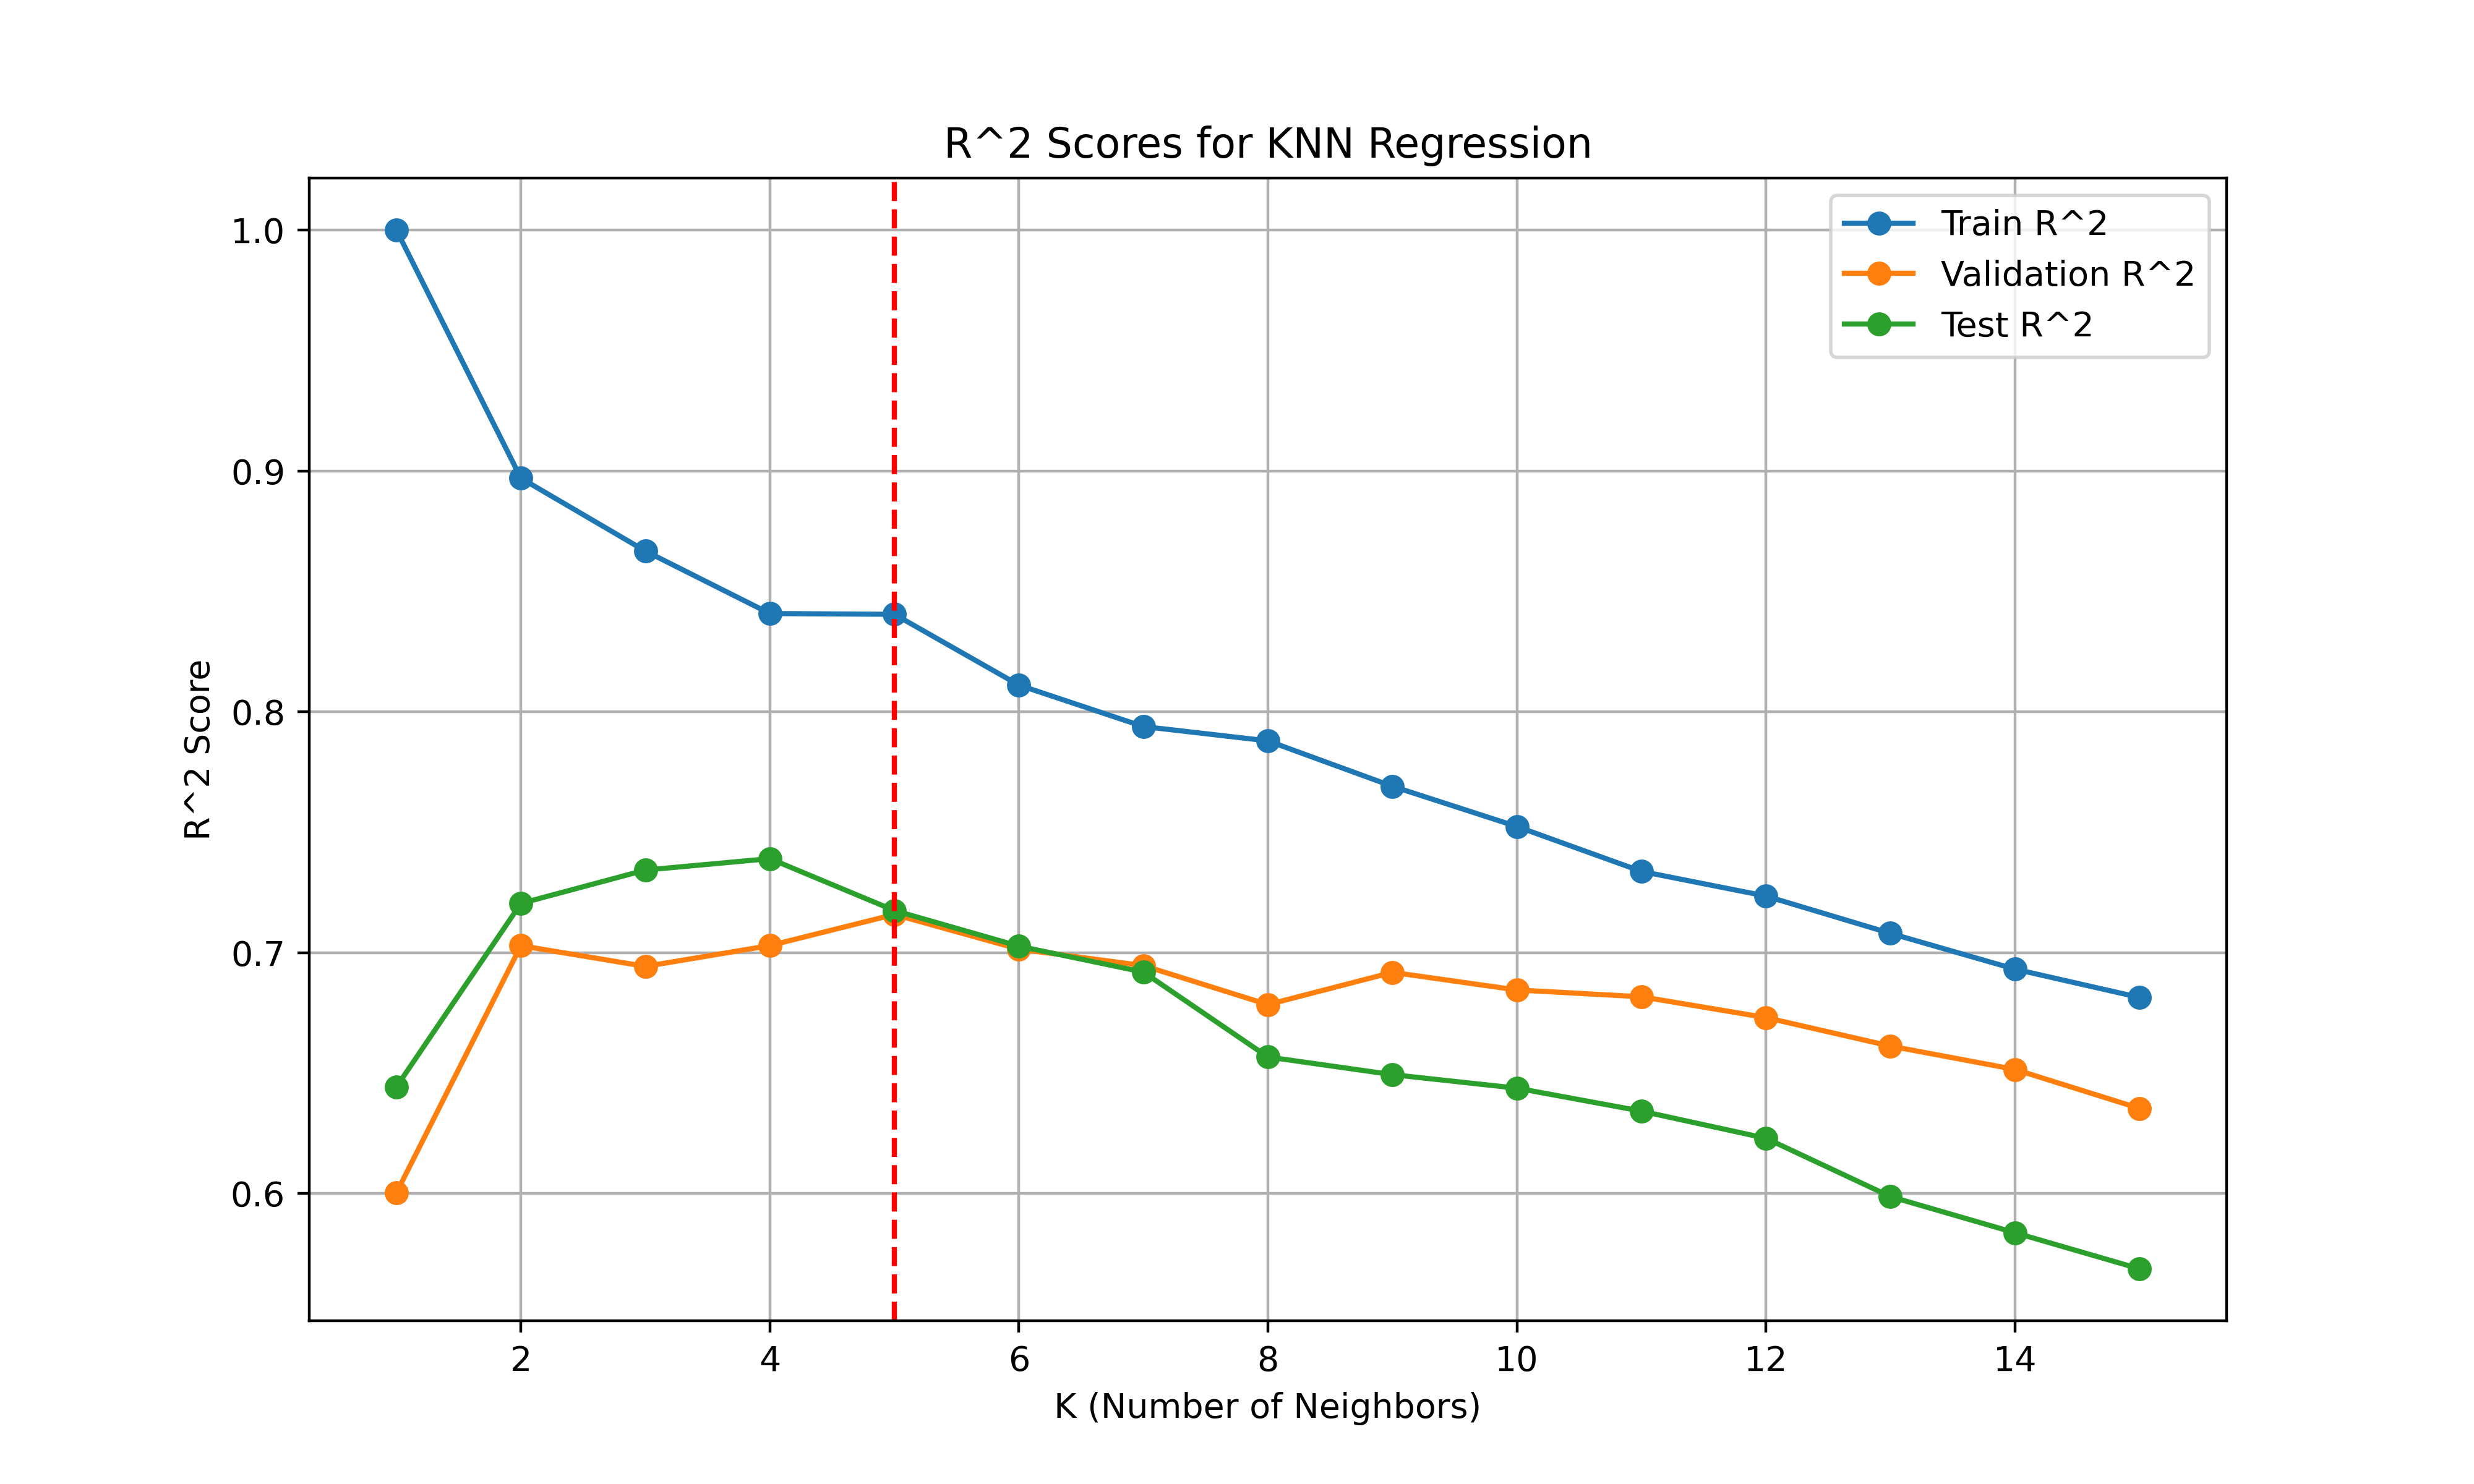
\includegraphics[width=1\textwidth]{Figure_HW3_42.png}
    \caption{R$^2$ Scores for KNN Regression as a function of $K$ (Parts A-F).}
    \label{fig:HW3_42}
\end{figure}



\subsection{$R^2$ vs K for Part G}
% Table: R^2 Scores for K=1 to 15
\begin{table}[H]
\centering
\begin{tabular}{|c|c|c|c|}
\hline
K & R$^2$ Train & R$^2$ Validation & R$^2$ Test \\
\hline
1  & 1.000000 & 0.716546 & 0.623767 \\
2  & 0.904653 & 0.776549 & 0.744325 \\
\textbf{3}  & \textbf{0.871593} & \textbf{0.783931} & \textbf{0.744019} \\
4  & 0.848981 & 0.766933 & 0.740847 \\
5  & 0.837591 & 0.746855 & 0.723288 \\
6  & 0.806427 & 0.745834 & 0.719918 \\
7  & 0.783856 & 0.740624 & 0.699558 \\
8  & 0.761016 & 0.746696 & 0.683261 \\
9  & 0.733154 & 0.737948 & 0.663566 \\
10 & 0.717842 & 0.708272 & 0.660512 \\
11 & 0.700236 & 0.690345 & 0.634689 \\
12 & 0.684627 & 0.669594 & 0.632212 \\
13 & 0.661533 & 0.656321 & 0.619422 \\
14 & 0.651624 & 0.658531 & 0.618147 \\
15 & 0.635750 & 0.650367 & 0.615527 \\
\hline
\end{tabular}
\caption{R$^2$ Scores for KNN Regression (K=1 to 15) for random state = 24. The best validation score is at $\mathbf{K=3}$.}
\label{tab:r2_scores_24}
\end{table}

\subsection{Visualizations Part G}
\begin{figure}[H]
    \centering
    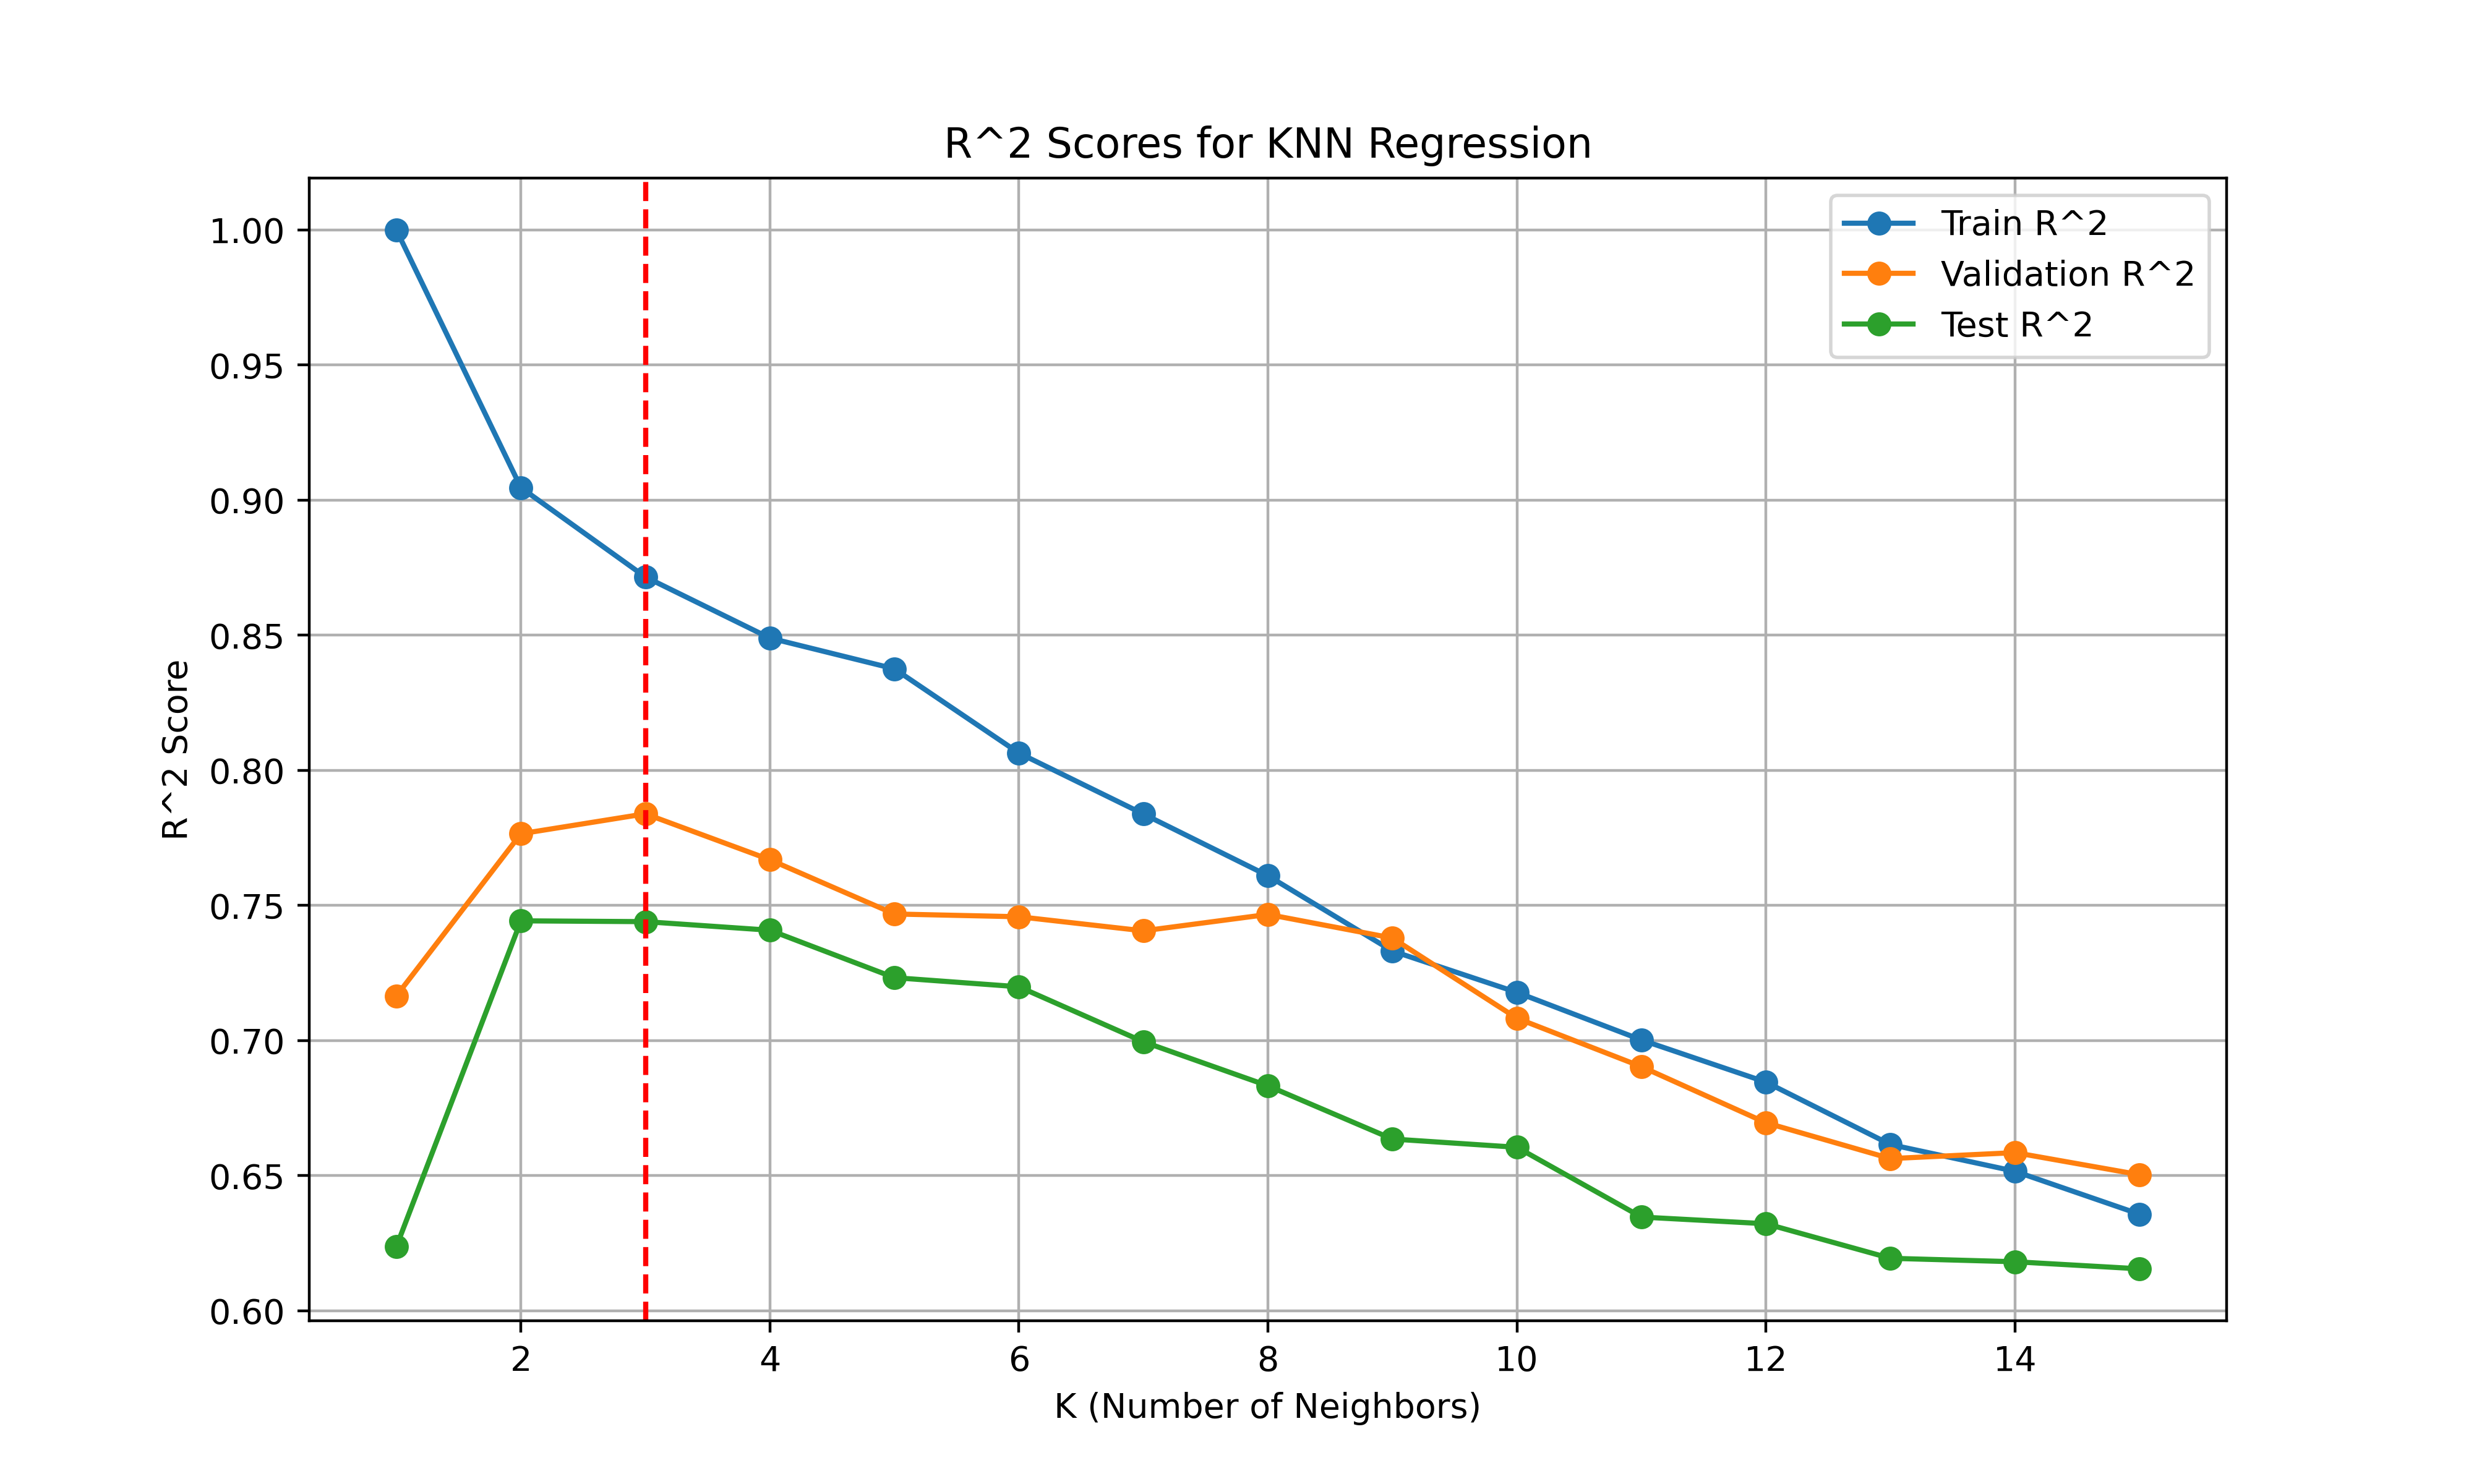
\includegraphics[width=1\textwidth]{Figure_HW3_24.png}
    \caption{R$^2$ Scores for KNN Regression as a function of $K$(Part G).}
    \label{fig:HW3_24}
\end{figure}


\section{Discussion}
For random state = 42; as shown in the visualization in (3.2) and the table in (3.1). The best value we found during training and prediction on the validation set was at K = 5 (Highlighted in Bold). Deemed the best since we we're choosing the best $R^2$ based off the validation set. As we progress through K's there is a noticeable drop in $R^2$ performance. At K = 1, it's overfit but once we get to K=4 and K=5 we reach the peak of our $R^2$'s for train/val/test, overall it explains 70 percent of the variance in the data. But then as we increase the size of K i.e. the number of neighbors the model considers. It starts to explain less and less in variability and then struggles to predict the test data. And this holds true for table (3.3) and the visualization (3.4) when toggling to random state=24. Considering a new split of data it shows roughly the same pattern. But the test and validation curves switch places and result in a K = 3 (Highlighted in Bold) as the best number of neighbors considered. Now, this means that there is a possibility for bias in the data that may be causing an effect on how the curves are calculated. This shows that the data split can influence which K is optimal and how sensitive a KNN is to data partitioning.


\section{Conclusion}
In conclusion, with the KNN regressor data partitioning and K selection matters. Since the neighbors the model considers during prediction is based off the training data that is given to it. Secondly, the value we select for K heavily affects the model's performance on the $R^2$ score metric, with different splits potentially yielding different optimal K values. Thus the choice to how much data is given and it's composition, plus the value of K we select for the model, will heavily determine the results we get for this regression. 

\section{Disclaimers}
\begin{itemize}
\item All Python code for data processing, model training, and visualization is available in the Jupyter notebook (\texttt{hw3.ipynb}).
    
\item This LaTeX document was formatted and generated by AI. All data, images and text were written in spaces by me to provide for a properly formatted report and ensure readability.
\end{itemize}
\end{document}
